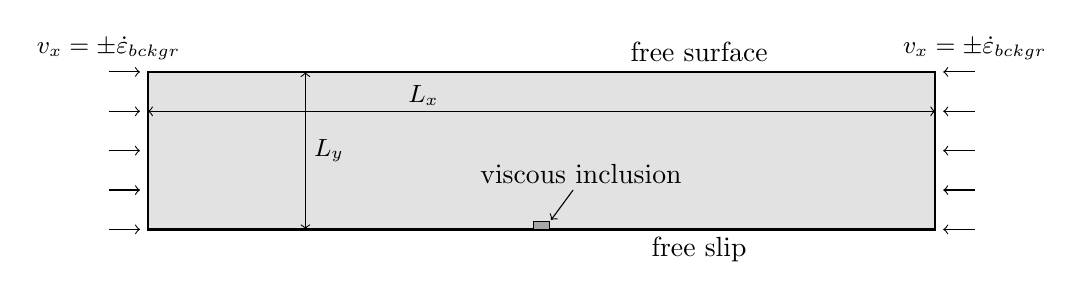
\begin{tikzpicture}
  \draw[fill=gray!23,gray!23](0,0) rectangle (10,2);
  %\draw[step=0.5cm,gray,very thin] (0,0) grid (10,8); %background grid
  
  % left part of drawing
  
  %domain
  \draw[fill=gray!23,thick](0,0) rectangle (10,2);
  %seed
  \draw[fill=gray!70](4.9,0) rectangle (5.1,0.1);
  %left arrows
  \draw [->] (-0.5,0) -- (-0.1,0);
  \draw [->] (-0.5,0.5) -- (-0.1,0.5);
  \draw [->] (-0.5,1) -- (-0.1,1);
  \draw [->] (-0.5,1.5) -- (-0.1,1.5);
  \draw [->] (-0.5,2) -- (-0.1,2);
  %right arrows
  \draw [<-] (10.1,0) -- (10.5,0);
  \draw [<-] (10.1,0.5) -- (10.5,0.5);
  \draw [<-] (10.1,1) -- (10.5,1);
  \draw [<-] (10.1,1.5) -- (10.5,1.5);
  \draw [<-] (10.1,2) -- (10.5,2);
  
  \node[] at (7,-0.25) {free slip};
  \node[] at (7,2.25) {free surface};
  
  \node[] at (-0.5,2.3) {\small $v_x=\pm \dot{\varepsilon}_{bckgr}$};
  \node[] at (10.5,2.3) {\small $v_x=\pm \dot{\varepsilon}_{bckgr}$};
  
  \draw [<-] (5.12,0.12) -- (5.4,0.5);
  \node[] at (5.5,0.7) {viscous inclusion};
  
  \draw [<->,thin] (0,1.5) -- (10,1.5);
  \node[] at (3.5,1.7) {\small $L_x$};
  
  \draw [<->,thin] (2,0) -- (2,2);
  \node[] at (2.3,1) {\small $L_y$};
  
  \end{tikzpicture}